% Options for packages loaded elsewhere
% Options for packages loaded elsewhere
\PassOptionsToPackage{unicode}{hyperref}
\PassOptionsToPackage{hyphens}{url}
%
\documentclass[
  ignorenonframetext,
  aspectratio=169,
]{beamer}
\newif\ifbibliography
\usepackage{pgfpages}
\setbeamertemplate{caption}[numbered]
\setbeamertemplate{caption label separator}{: }
\setbeamercolor{caption name}{fg=normal text.fg}
\beamertemplatenavigationsymbolsempty
% remove section numbering
\setbeamertemplate{part page}{
  \centering
  \begin{beamercolorbox}[sep=16pt,center]{part title}
    \usebeamerfont{part title}\insertpart\par
  \end{beamercolorbox}
}
\setbeamertemplate{section page}{
  \centering
  \begin{beamercolorbox}[sep=12pt,center]{section title}
    \usebeamerfont{section title}\insertsection\par
  \end{beamercolorbox}
}
\setbeamertemplate{subsection page}{
  \centering
  \begin{beamercolorbox}[sep=8pt,center]{subsection title}
    \usebeamerfont{subsection title}\insertsubsection\par
  \end{beamercolorbox}
}
% Prevent slide breaks in the middle of a paragraph
\widowpenalties 1 10000
\raggedbottom
\usepackage{iftex}
\ifPDFTeX
  \usepackage[T1]{fontenc}
  \usepackage[utf8]{inputenc}
  \usepackage{textcomp} % provide euro and other symbols
\else % if luatex or xetex
  \usepackage{unicode-math} % this also loads fontspec
  \defaultfontfeatures{Scale=MatchLowercase}
  \defaultfontfeatures[\rmfamily]{Ligatures=TeX,Scale=1}
\fi
\usepackage{lmodern}

\ifPDFTeX\else
  % xetex/luatex font selection
\fi
% Use upquote if available, for straight quotes in verbatim environments
\IfFileExists{upquote.sty}{\usepackage{upquote}}{}
\IfFileExists{microtype.sty}{% use microtype if available
  \usepackage[]{microtype}
  \UseMicrotypeSet[protrusion]{basicmath} % disable protrusion for tt fonts
}{}
\makeatletter
\@ifundefined{KOMAClassName}{% if non-KOMA class
  \IfFileExists{parskip.sty}{%
    \usepackage{parskip}
  }{% else
    \setlength{\parindent}{0pt}
    \setlength{\parskip}{6pt plus 2pt minus 1pt}}
}{% if KOMA class
  \KOMAoptions{parskip=half}}
\makeatother


\usepackage{longtable,booktabs,array}
\usepackage{calc} % for calculating minipage widths
\usepackage{caption}
% Make caption package work with longtable
\makeatletter
\def\fnum@table{\tablename~\thetable}
\makeatother
\usepackage{graphicx}
\makeatletter
\newsavebox\pandoc@box
\newcommand*\pandocbounded[1]{% scales image to fit in text height/width
  \sbox\pandoc@box{#1}%
  \Gscale@div\@tempa{\textheight}{\dimexpr\ht\pandoc@box+\dp\pandoc@box\relax}%
  \Gscale@div\@tempb{\linewidth}{\wd\pandoc@box}%
  \ifdim\@tempb\p@<\@tempa\p@\let\@tempa\@tempb\fi% select the smaller of both
  \ifdim\@tempa\p@<\p@\scalebox{\@tempa}{\usebox\pandoc@box}%
  \else\usebox{\pandoc@box}%
  \fi%
}
% Set default figure placement to htbp
\def\fps@figure{htbp}
\makeatother





\setlength{\emergencystretch}{3em} % prevent overfull lines

\providecommand{\tightlist}{%
  \setlength{\itemsep}{0pt}\setlength{\parskip}{0pt}}



 


% ============================================================
%  ECO 2203 — Beamer Metropolis Theme Preamble
%  Course: International Trade and Policy in Agriculture
%  Instructor: Nithin M, Department of Development Economics
% ============================================================

% MUST be first: load Metropolis theme before \metroset and colour overrides
\usetheme{metropolis}

% Only load packages not already provided by pandoc's beamer template
\usepackage{amsmath,amssymb}

% ---- Brand colours -----------------------------------------
\definecolor{brandblue}{HTML}{012169}
\definecolor{brandgold}{HTML}{B9975B}
\definecolor{lightblue}{HTML}{E8EDF5}

% ---- Metropolis colour overrides ---------------------------
% Main palette
\setbeamercolor{normal text}{fg=black,bg=white}
\setbeamercolor{alerted text}{fg=brandgold}
\setbeamercolor{example text}{fg=brandblue!70!black}

% Title slide
\setbeamercolor{title}{fg=white,bg=brandblue}
\setbeamercolor{subtitle}{fg=brandgold}
\setbeamercolor{author}{fg=white}
\setbeamercolor{institute}{fg=brandgold!80!white}
\setbeamercolor{date}{fg=white}
\setbeamercolor{title page header}{fg=white,bg=brandblue}

% Frametitle bar
\setbeamercolor{frametitle}{fg=white,bg=brandblue}

% Progress bar → gold
\setbeamercolor{progress bar}{fg=brandgold,bg=brandblue!30}
\setbeamercolor{title separator}{fg=brandgold}
\setbeamercolor{progress bar in head/foot}{fg=brandgold,bg=brandblue!20}
\setbeamercolor{progress bar in section page}{fg=brandgold,bg=brandblue!20}

% Blocks
\setbeamercolor{block title}{bg=brandblue,fg=white}
\setbeamercolor{block body}{bg=lightblue,fg=black}
\setbeamercolor{block title alerted}{bg=brandgold,fg=white}
\setbeamercolor{block body alerted}{bg=brandgold!12,fg=black}
\setbeamercolor{block title example}{bg=brandblue!70!black,fg=white}
\setbeamercolor{block body example}{bg=brandblue!8,fg=black}

% Structure / lists
\setbeamercolor{structure}{fg=brandblue}
\setbeamercolor{section in toc}{fg=brandblue}
\setbeamercolor{itemize item}{fg=brandblue}
\setbeamercolor{itemize subitem}{fg=brandgold}
\setbeamercolor{enumerate item}{fg=brandblue}
\setbeamercolor{description item}{fg=brandblue}

% ---- Metropolis options ------------------------------------
\metroset{
  progressbar    = frametitle,   % gold bar under frametitle
  sectionpage    = none,
  numbering      = fraction,
  block          = fill
}

% ---- Fonts (Metropolis uses Fira Sans; fallback gracefully) -
\setbeamerfont{title}{size=\Large,series=\bfseries}
\setbeamerfont{subtitle}{size=\normalsize,series=\mdseries}
\setbeamerfont{frametitle}{size=\large,series=\bfseries}
\setbeamerfont{block title}{size=\normalsize,series=\bfseries}
\setbeamerfont{caption}{size=\footnotesize}

% ---- Footer: course info + slide number --------------------
\setbeamertemplate{footline}{%
  \begin{beamercolorbox}[wd=\paperwidth,ht=2.0ex,dp=1ex]{footline}%
    \hspace{0.8em}%
    {\footnotesize\color{brandblue!60}%
      ECO 2203 \textbar{} International Trade and Policy in Agriculture
      \hfill Nithin M \hfill
      \insertframenumber{}/\inserttotalframenumber\hspace{0.8em}}%
  \end{beamercolorbox}%
}

% ---- Misc --------------------------------------------------
\setlength{\parskip}{0.25em}
\setbeamertemplate{navigation symbols}{}

% tighter column sep for side-by-side content
\setlength{\columnsep}{0.8em}

% Fix: make \label truly robust in moving arguments (Quarto generates
% \caption{\label{fig-xxx}...} which crashes Metropolis in batchmode).
% DeclareRobustCommand creates a self-protecting robust version.
\makeatletter
\let\quarto@originallabel\label
\DeclareRobustCommand*{\label}[1]{\quarto@originallabel{#1}}
\makeatother

% Prevent figures from overflowing Beamer frames.
% width=\linewidth: scale to text width (already Quarto default);
% height=0.6\textheight: cap height so figures never push past the frame bottom.
% keepaspectratio: never distort — whichever constraint binds first wins.
\setkeys{Gin}{width=\linewidth,height=0.6\textheight,keepaspectratio}
\makeatletter
\@ifpackageloaded{caption}{}{\usepackage{caption}}
\AtBeginDocument{%
\ifdefined\contentsname
  \renewcommand*\contentsname{Table of contents}
\else
  \newcommand\contentsname{Table of contents}
\fi
\ifdefined\listfigurename
  \renewcommand*\listfigurename{List of Figures}
\else
  \newcommand\listfigurename{List of Figures}
\fi
\ifdefined\listtablename
  \renewcommand*\listtablename{List of Tables}
\else
  \newcommand\listtablename{List of Tables}
\fi
\ifdefined\figurename
  \renewcommand*\figurename{Figure}
\else
  \newcommand\figurename{Figure}
\fi
\ifdefined\tablename
  \renewcommand*\tablename{Table}
\else
  \newcommand\tablename{Table}
\fi
}
\@ifpackageloaded{float}{}{\usepackage{float}}
\floatstyle{ruled}
\@ifundefined{c@chapter}{\newfloat{codelisting}{h}{lop}}{\newfloat{codelisting}{h}{lop}[chapter]}
\floatname{codelisting}{Listing}
\newcommand*\listoflistings{\listof{codelisting}{List of Listings}}
\makeatother
\makeatletter
\makeatother
\makeatletter
\@ifpackageloaded{caption}{}{\usepackage{caption}}
\@ifpackageloaded{subcaption}{}{\usepackage{subcaption}}
\makeatother

\usepackage{bookmark}
\IfFileExists{xurl.sty}{\usepackage{xurl}}{} % add URL line breaks if available
\urlstyle{same}
\hypersetup{
  pdftitle={Lecture 14: Agreement on Agriculture},
  pdfauthor={Nithin M},
  hidelinks,
  pdfcreator={LaTeX via pandoc}}


\title{Lecture 14: Agreement on Agriculture}
\subtitle{ECO 2203 \textbar{} International Trade and Policy in
Agriculture}
\author{Nithin M}
\date{2026-07-25}
\institute{Department of Development Economics}

\begin{document}
\frame{\titlepage}


\begin{frame}{Recap: Lecture 13}
\phantomsection\label{recap-lecture-13}
\textbf{Lecture 13} established the WTO as the institutional framework
of international trade.

\begin{columns}[T]
\begin{column}{0.55\linewidth}
\textbf{Key ideas from Lecture 13:}

\begin{itemize}
\tightlist
\item
  GATT → WTO (1995): from provisional to permanent
\item
  Five core principles: MFN, National Treatment, Bound Tariffs,
  Reciprocity, Transparency
\item
  DSU: binding dispute settlement
\item
  India's Peace Clause --- protects MSP procurement
\item
  Doha Round stalemate: agriculture at the core
\end{itemize}
\end{column}

\begin{column}{0.45\linewidth}
\textbf{Today's Focus}

We zoom into the \textbf{Agreement on Agriculture (AoA)} --- the
specific WTO text that governs how much protection India can give its
farmers, how much support the US/EU can give theirs, and how
agricultural trade is managed globally.

Three pillars: \textbf{Market Access · Domestic Support · Export
Competition}
\end{column}
\end{columns}
\end{frame}

\begin{frame}{Why Was the AoA Needed?}
\phantomsection\label{why-was-the-aoa-needed}
\begin{columns}[T]
\begin{column}{0.55\linewidth}
\textbf{Pre-Uruguay Round Agriculture: A Wild West}

Before 1995, agriculture was essentially \textbf{outside GATT
discipline}:

\begin{itemize}
\tightlist
\item
  USA had a 1955 GATT waiver exempting its agricultural support programs
\item
  EU's Common Agricultural Policy (CAP): massive production and export
  subsidies
\item
  Result: \textbf{global overproduction} of wheat, butter, sugar;
  chronic dumping on world markets
\end{itemize}

\textbf{The dumping problem:} In the 1980s, EU butter was sold on world
markets at 20\% of EU domestic prices. US wheat exports were subsidised
by up to 40\%. This depressed world prices and \textbf{hurt farmers in
Australia, Argentina, Brazil, India, and the developing world}.
\end{column}

\begin{column}{0.45\linewidth}
\textbf{Why This Hurt India}

Artificially low world prices for wheat and rice: - Made Indian exports
uncompetitive - Provided cheap food imports that undercut domestic
prices - Reduced incentives for agricultural investment globally

The AoA's promise to the developing world: - \textbf{Discipline} US/EU
subsidies - \textbf{Reduce} import barriers - \textbf{Eliminate} export
subsidies

Reality: progress has been slow --- but the framework now exists.
\end{column}
\end{columns}
\end{frame}

\begin{frame}{AoA Structure: The Three Pillars + S\&DT}
\phantomsection\label{aoa-structure-the-three-pillars-sdt}
\textbf{Agreement on Agriculture (1995) --- 21 Articles + Annexes} In
force: January 1, 1995 \textbar{} Implementation period: 1995--2004
(developed), 1995--2005 (developing)

\begin{columns}[T]
\begin{column}{0.5\linewidth}
\textbf{Agreement on Agriculture (1995)}

\begin{itemize}
\tightlist
\item
  \textbf{Pillar 1: Market Access}

  \begin{itemize}
  \tightlist
  \item
    Tariffication of non-tariff barriers
  \item
    Bound tariff schedules
  \item
    Tariff reduction commitments (average 36\%)
  \item
    Minimum access provisions (3--5\% of domestic consumption)
  \item
    Special Safeguard (SSG) clause
  \end{itemize}
\item
  \textbf{Pillar 2: Domestic Support}

  \begin{itemize}
  \tightlist
  \item
    Aggregate Measurement of Support (AMS) reduction (20\% for
    developed, 13.3\% for developing)
  \item
    Green Box: non-distorting (exempt)
  \item
    Blue Box: production-limiting (exempt)
  \item
    Amber Box: trade-distorting (limited)
  \item
    De minimis provisions
  \end{itemize}
\item
  \textbf{Pillar 3: Export Competition}

  \begin{itemize}
  \tightlist
  \item
    Export subsidy reduction/elimination
  \item
    Export credit disciplines
  \end{itemize}
\end{itemize}
\end{column}

\begin{column}{0.5\linewidth}
\textbf{Special and Differential Treatment (S\&DT)}

Developing countries get: - Longer implementation periods (10 vs.~6
years) - Smaller reduction commitments (24\% vs.~36\% tariff cuts; 13\%
vs.~24\% domestic support cuts) - Higher de minimis thresholds (10\%
vs.~5\%) - Continued input subsidies for poor farmers - Continued
investment subsidies for agricultural development

\textbf{India fully utilises all S\&DT provisions}
\end{column}
\end{columns}
\end{frame}

\begin{frame}
\end{frame}

\section{Pillar 1 --- Market Access}\label{pillar-1-market-access}

\begin{frame}{Tariffication: Converting NTBs to Tariffs}
\phantomsection\label{tariffication-converting-ntbs-to-tariffs}
\begin{columns}[T]
\begin{column}{0.55\linewidth}
\textbf{What is Tariffication?}

Before 1995: Countries protected agriculture through: - Import quotas
(how much can come in) - Variable levies (duty adjusts to keep domestic
prices stable) - Minimum import prices - Voluntary export restraints

AoA Article 4: \textbf{All these NTBs converted to tariff equivalents}
(bound tariff rates in WTO schedules) by 1995.

\textbf{The Reduction Commitment:}

\begin{longtable}[]{@{}llll@{}}
\toprule\noalign{}
Country & Average Cut & Minimum/Product & Period \\
\midrule\noalign{}
\endhead
Developed & 36\% & 15\% & 6 years \\
Developing & 24\% & 10\% & 10 years \\
LDCs & None & None & --- \\
\bottomrule\noalign{}
\end{longtable}
\end{column}

\begin{column}{0.45\linewidth}
\textbf{``Dirty Tariffication''}

Many developed countries set artificially \textbf{high tariff
equivalents} when converting their NTBs --- overstating the protection
level to preserve policy space.

Example: Canada's tariff on butter: \textbf{298\%}; on chicken:
\textbf{238\%}

This gave rich countries huge ``water in the tariff'' even after the
required cuts.

India negotiated high bound rates (113\% average) for similar reasons
--- policy space for future flexibility.
\end{column}
\end{columns}
\end{frame}

\begin{frame}{AoA Tariff Reduction Commitments}
\phantomsection\label{aoa-tariff-reduction-commitments}
\begin{figure}

\centering{

\pandocbounded{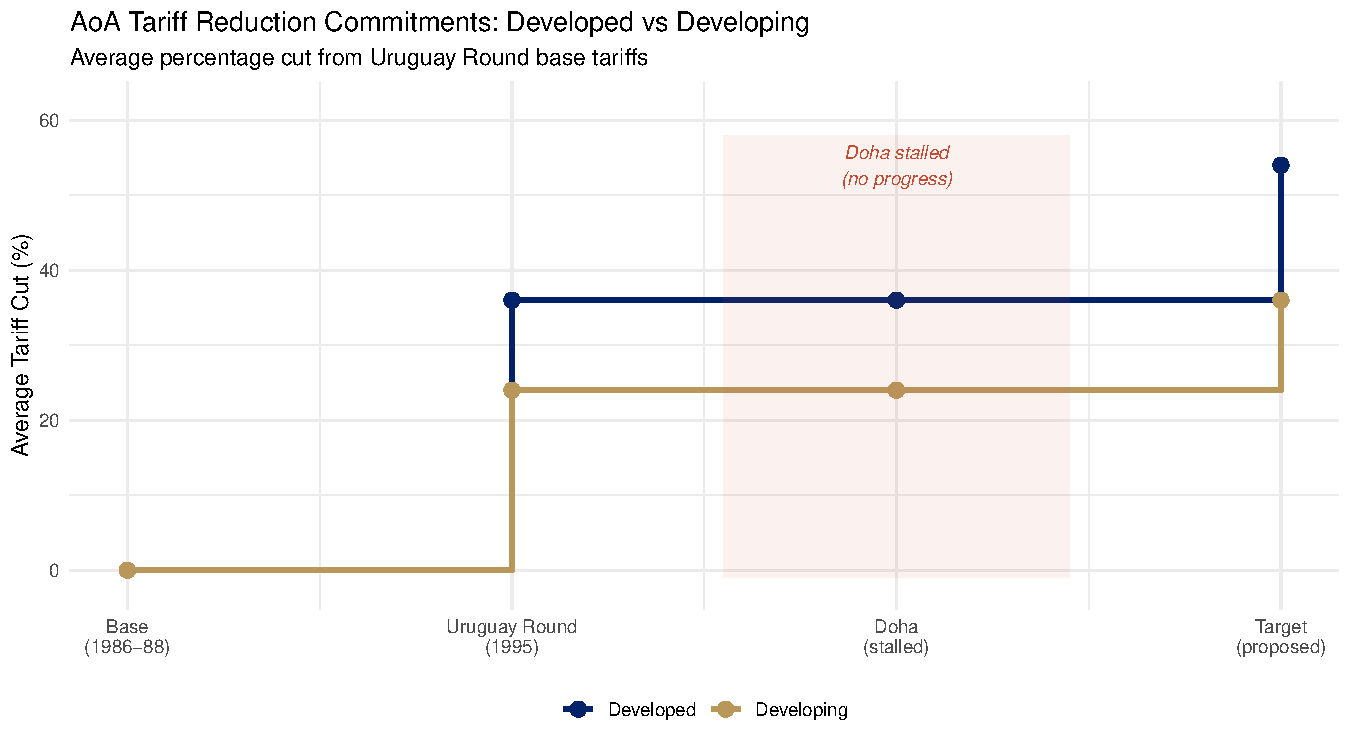
\includegraphics[keepaspectratio]{Lecture14_Agreement_on_Agriculture_files/figure-beamer/fig-aoa-tariff-reduction-1.pdf}}

}

\caption{\label{fig-aoa-tariff-reduction}AoA Tariff Reduction
Commitments: Developed vs Developing Source: WTO, Agreement on
Agriculture; UNCTAD.}

\end{figure}%
\end{frame}

\begin{frame}[fragile]{Tariff Rate Quotas (TRQs)}
\phantomsection\label{tariff-rate-quotas-trqs}
\begin{columns}[T]
\begin{column}{0.55\linewidth}
\textbf{How TRQs Work}

Where post-tariffication tariffs were extremely high, \textbf{TRQs} were
created to ensure minimum market access:

\begin{itemize}
\tightlist
\item
  \textbf{In-quota tariff:} lower rate (e.g., 15\%) applied to a
  specified quantity
\item
  \textbf{Out-of-quota tariff:} higher rate (e.g., 60\%) applied to
  quantities above the quota
\end{itemize}

\begin{verbatim}
Imports
  ↑
  │ Out-of-quota tariff = 60%
  │ ───────────────────────────
  │ In-quota tariff = 15%     ← TRQ fills here
  └─────────────────────────→ Volume
        Quota quantity
\end{verbatim}

\textbf{Minimum access commitment:} 5\% of domestic consumption by end
of implementation period
\end{column}

\begin{column}{0.45\linewidth}
\textbf{India's TRQ Commitments}

India has TRQs for:

\begin{longtable}[]{@{}lll@{}}
\toprule\noalign{}
Product & In-quota rate & Out-of-quota \\
\midrule\noalign{}
\endhead
Wheat & 50\% & 100\% \\
Rice (non-PDS) & 70\% & 80\% \\
Maize & 15\% & 60\% \\
Sunflower oil & 100\% & 100\% \\
Cotton & 5\% & 10\% \\
\bottomrule\noalign{}
\end{longtable}

\textbf{Most Indian TRQ quotas are never filled} --- because even the
in-quota tariff is high enough to limit imports below the quota. India's
TRQs are symbolic: the real protection is the bound tariff, not the TRQ.
\end{column}
\end{columns}
\end{frame}

\begin{frame}{India's Bound Tariffs: Agricultural Products}
\phantomsection\label{indias-bound-tariffs-agricultural-products}
\begin{columns}[T]
\begin{column}{0.5\linewidth}
\textbf{``Water in the Tariff'' --- India's Policy Flexibility}

\begin{longtable}[]{@{}llll@{}}
\toprule\noalign{}
Product & Bound (\%) & Applied (2024, \%) & Water (\%) \\
\midrule\noalign{}
\endhead
Rice & 80 & 25 & \textbf{55} \\
Wheat & 100 & 40 & \textbf{60} \\
Maize & 60 & 50 & \textbf{10} \\
Sugar & 150 & 100 & \textbf{50} \\
Crude palm oil & 300 & 100 & \textbf{200} \\
Refined palm oil & 300 & 100 & \textbf{200} \\
Chickpeas & 100 & 50 & \textbf{50} \\
Milk powder (SMP) & 60 & 30 & \textbf{30} \\
Onions & 100 & 0 & \textbf{100} \\
\bottomrule\noalign{}
\end{longtable}
\end{column}

\begin{column}{0.5\linewidth}
\textbf{How India Used This Space --- Palm Oil}

In 2018--19, domestic oilseed farmers (soybean, groundnut, sunflower)
were hurt by cheap imported palm oil from Malaysia and Indonesia.

India \textbf{raised the applied tariff} on crude palm oil from 30\% to
100\% (still below bound 300\%).

This protected domestic edible oil industry without violating WTO --- no
dispute case possible.

Then in 2021, India \textbf{lowered it again} to reduce consumer food
prices during inflation. Flexible policy instrument.

The large tariff ``water'' is India's most important defensive trade
policy instrument for agriculture
\end{column}
\end{columns}
\end{frame}

\begin{frame}{Special Safeguard (SSG) vs.~SSM}
\phantomsection\label{special-safeguard-ssg-vs.-ssm}
\begin{columns}[T]
\begin{column}{0.55\linewidth}
\textbf{Special Safeguard (SSG) --- AoA Article 5}

Allows additional tariff duties \textbf{automatically} (no injury
investigation needed) when: - \textbf{Volume trigger:} imports exceed
125\% of average imports in previous 3 years; OR - \textbf{Price
trigger:} import price falls more than 10\% below average 1986--88 price

\textbf{Only available to countries that tariffied their NTBs} ---
mainly developed countries and a few developing countries that had NTBs
pre-1995.

India cannot invoke the SSG on most products because India used high
bound tariffs, not tariffication of all NTBs. India has SSG access for
only \textasciitilde6 products.
\end{column}

\begin{column}{0.45\linewidth}
\textbf{Special Safeguard Mechanism (SSM)}

\textbf{What developing countries want (Doha)}

An SSM would allow all developing countries to temporarily raise tariffs
beyond bound levels when imports surge or prices fall --- without the
SSG's historical eligibility restriction.

Key disagreement (2008 collapse): At what threshold can the SSM be
triggered? USA wanted 140\% of import volume; India demanded 110\%.

\textbf{SSM not agreed} --- one of the main reasons the Doha Round
collapsed.
\end{column}
\end{columns}
\end{frame}

\begin{frame}
\end{frame}

\section{Pillar 2 --- Domestic Support}\label{pillar-2-domestic-support}

\begin{frame}{Aggregate Measurement of Support (AMS)}
\phantomsection\label{aggregate-measurement-of-support-ams}
\begin{columns}[T]
\begin{column}{0.55\linewidth}
\textbf{What is AMS?}

A measure of the total trade-distorting domestic support given to
agriculture by a government.

\textbf{Formula for product-specific AMS:}

\[\text{AMS} = (\text{Administered Price} - \text{FERP}) \times \text{Eligible Production}\]

where: - \textbf{Administered Price} = MSP or procurement price -
\textbf{FERP} = Fixed External Reference Price (average world price,
1986--88) - \textbf{Eligible Production} = quantity actually purchased
at administered price

\textbf{Non-product-specific AMS:} Sum of general input subsidies
(fertiliser, power, irrigation, credit) across all crops
\end{column}

\begin{column}{0.45\linewidth}
\textbf{Why the FERP is controversial}

The FERP is fixed at \textbf{1986--88 world prices} --- when US and EU
subsidies were at their peak, artificially depressing world prices.

Rice FERP: \textbf{USD 116/tonne} (1986--88 world price)

Current world price (2024): \textasciitilde{}\textbf{USD 450--500/tonne}

So the ``ceiling'' against which India's MSP is measured is a
40-year-old, distorted baseline. India argues this systematically
overestimates India's support and underestimates rich country support.

Developing country de minimis: \textbf{10\%} of production value (5\%
for developed countries)
\end{column}
\end{columns}
\end{frame}

\begin{frame}{The Three Boxes: Traffic Light Analogy}
\phantomsection\label{the-three-boxes-traffic-light-analogy}
\begin{columns}[T]
\begin{column}{0.33\linewidth}
\textbf{🟢 GREEN BOX}

\emph{Allowed --- no limit}

Criteria: - Government-funded - No price support - Minimal trade
distortion

Includes: - Agricultural research - Extension services - Pest/disease
control - Infrastructure - Food security stockholding (with conditions)
- Decoupled income support - Environmental programs
\end{column}

\begin{column}{0.33\linewidth}
\textbf{🔵 BLUE BOX}

\emph{Permitted conditionally}

Payments under \textbf{production-limiting programs}

Used primarily by EU (old area payments) and USA (counter-cyclical
payments tied to historical acreage, not current production)

Less relevant for India --- India doesn't formally claim Blue Box,
though some argue certain schemes could qualify
\end{column}

\begin{column}{0.33\linewidth}
\textbf{🟡 AMBER BOX}

\emph{Restricted --- must not exceed AMS commitment}

All trade-distorting support: MSP procurement, input price subsidies
tied to specific products

Subject to de minimis threshold: - Product-specific: 10\% of that
product's value - Non-product-specific: 10\% of total agri output value

India's AMS commitment: India has no scheduled AMS reduction commitment
--- it must only stay within de minimis (10\%)
\end{column}
\end{columns}
\end{frame}

\begin{frame}{India's Agricultural Support by WTO Box}
\phantomsection\label{indias-agricultural-support-by-wto-box}
\begin{figure}

\centering{

\pandocbounded{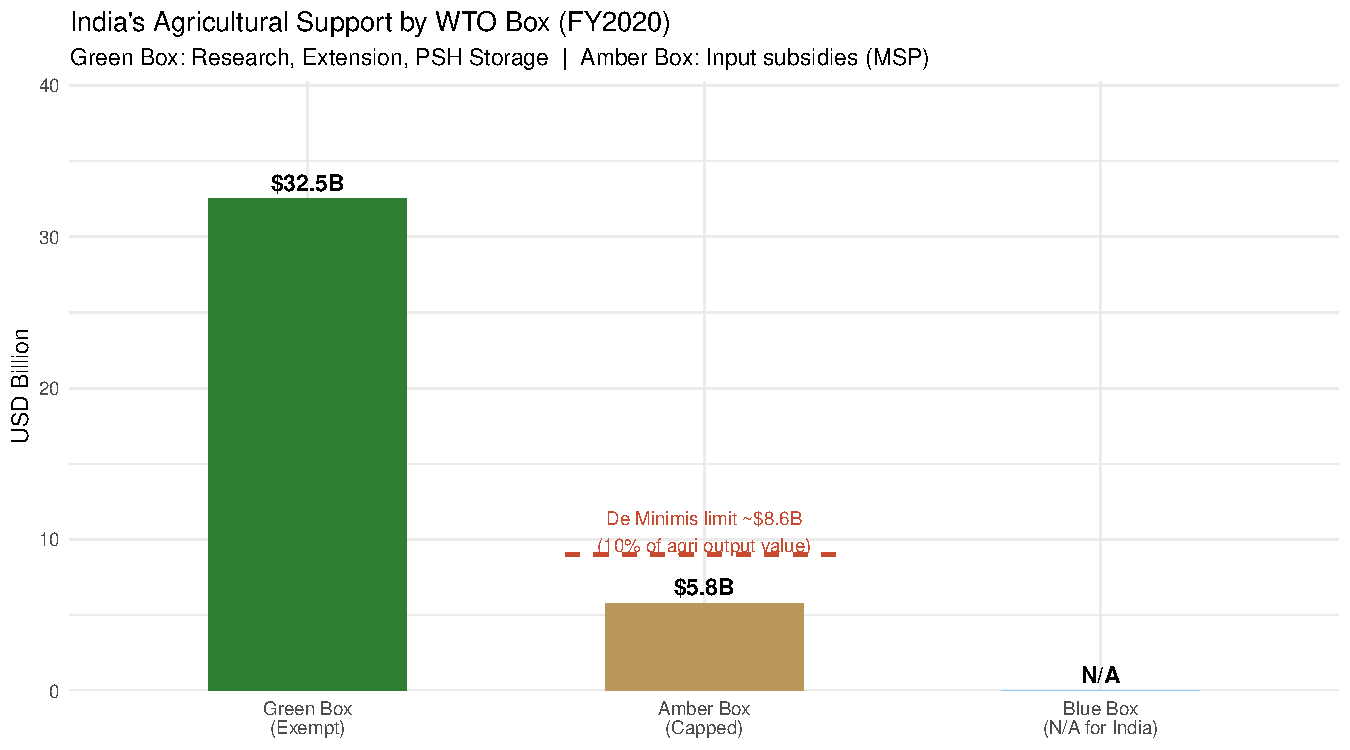
\includegraphics[keepaspectratio]{Lecture14_Agreement_on_Agriculture_files/figure-beamer/fig-india-box-subsidies-1.pdf}}

}

\caption{\label{fig-india-box-subsidies}India's Agricultural Support by
WTO Box (FY2020) Source: India's WTO Domestic Support Notifications;
Ministry of Agriculture, GoI.}

\end{figure}%
\end{frame}

\begin{frame}{Green Box: What India Can and Cannot Claim}
\phantomsection\label{green-box-what-india-can-and-cannot-claim}
\begin{columns}[T]
\begin{column}{0.55\linewidth}
\textbf{India's Legitimate Green Box Programs}

Programs India can legitimately classify as Green Box:

\begin{itemize}
\tightlist
\item
  \textbf{ICAR research programs} --- rice varieties, disease
  resistance, HYV seeds
\item
  \textbf{Krishi Vigyan Kendras (KVKs)} --- 731 farm science centres
  across India
\item
  \textbf{Agricultural extension services} --- ATMA, ARYA programs
\item
  \textbf{National Food Security Act} --- \emph{food security
  stockholding} (subject to conditions)
\item
  \textbf{Pradhan Mantri Krishi Sinchayee Yojana} --- irrigation
  infrastructure
\item
  \textbf{PM-KISAN} --- ₹6,000/year decoupled income transfer to 110
  million farmers
\item
  \textbf{Crop insurance (PMFBY)} --- part may qualify as decoupled
\end{itemize}
\end{column}

\begin{column}{0.45\linewidth}
\textbf{What India CANNOT Claim as Green Box}

\textbf{MSP procurement system} is NOT Green Box because:

\begin{enumerate}
\tightlist
\item
  It involves price support (FCI buys at above-market MSP)
\item
  It is linked to the quantity produced and sold to government
\item
  It distorts production decisions --- farmers produce more rice/wheat
  for FCI procurement than they would at market prices
\end{enumerate}

→ MSP procurement falls in the \textbf{Amber Box} → Subject to de
minimis limit → Protected only by Peace Clause

PM-KISAN, if truly decoupled (paid regardless of what crop is grown or
how much), is a legitimate Green Box payment. India has been expanding
this.
\end{column}
\end{columns}
\end{frame}

\begin{frame}{India's Amber Box Challenge: The Numbers}
\phantomsection\label{indias-amber-box-challenge-the-numbers}
\begin{columns}[T]
\begin{column}{0.55\linewidth}
\textbf{Calculating India's Rice AMS (FY2023--24)}

\begin{longtable}[]{@{}ll@{}}
\toprule\noalign{}
Item & Value \\
\midrule\noalign{}
\endhead
MSP for paddy (common) & ₹2,183/quintal ≈ \textbf{USD 26.3/quintal} \\
FERP (1986--88 world price) & USD 116/tonne = \textbf{USD
11.6/quintal} \\
Support per quintal & USD 26.3 − USD 11.6 = \textbf{USD 14.7/quintal} \\
Total procurement by FCI & \textasciitilde{}\textbf{42 million
tonnes} \\
\textbf{Total rice AMS} & USD 14.7 × 420,000 quintals per
tonne\ldots{} \\
\bottomrule\noalign{}
\end{longtable}

Calculation: USD 14.7/quintal × 420 million quintals =
\textbf{\textasciitilde USD 6.2 billion}

De minimis limit (10\% of rice production value): Rice output
\textasciitilde120 MT × \textasciitilde USD 250/tonne = USD 30B × 10\% =
\textbf{\textasciitilde USD 3 billion threshold}

India's rice AMS (\textbf{USD 6.2B}) \textbf{exceeds} the de minimis
limit (\textbf{USD 3B})
\end{column}

\begin{column}{0.45\linewidth}
\textbf{Why India Is Technically in Violation}

India's rice AMS exceeds its 10\% de minimis limit. Without the Peace
Clause:

→ Any WTO member could bring a dispute case → Panel could find India in
violation → India would need to either cut MSP or reduce procurement

This is why the \textbf{Peace Clause is not optional for India} --- it
is existential for India's food security architecture.

\textbf{India's counter-argument:} Update the FERP to current world
prices. AMS would then be \textbf{negative} (MSP \textless{} current
world price for rice and wheat).
\end{column}
\end{columns}
\end{frame}

\begin{frame}{Peace Clause: Technical Details}
\phantomsection\label{peace-clause-technical-details}
\begin{columns}[T]
\begin{column}{0.55\linewidth}
\textbf{Bali Ministerial Decision on Public Stockholding} \emph{(MC9,
December 2013 --- India's biggest recent WTO win)}

\textbf{Conditions for Peace Clause protection:}

\begin{enumerate}
\tightlist
\item
  Program \textbf{existed before December 31, 2013} (India's FCI
  procurement qualifies)
\item
  \textbf{Annual notification} to WTO Committee on Agriculture with
  detailed data on:

  \begin{itemize}
  \tightlist
  \item
    Stocks procured, average prices, distribution
  \item
    Assessment of trade distortion impact
  \end{itemize}
\item
  Stocks \textbf{not exported below acquisition cost} --- cannot be used
  to dump food on world markets
\item
  Program \textbf{targets the poor} --- National Food Security Act 2013
  explicitly does this (75\% rural, 50\% urban population)
\end{enumerate}

India has notified its public stockholding program \textbf{every year}
since 2013
\end{column}

\begin{column}{0.45\linewidth}
\textbf{The Permanent Solution Problem}

MC10 Nairobi (2015): ``Ministerial Decision affirms that the Peace
Clause will remain in force until a permanent solution is found.''

Committed to permanent solution by \textbf{MC11 (2017)} --- missed.

Each subsequent MC: reaffirmed commitment --- no solution.

India's demands for permanent solution: 1. Update FERP to current world
prices OR base year of 2014--16 2. Include food inflation adjustment 3.
No conditions on which crops qualify

The FERP update would essentially solve India's problem --- at current
world prices, India's MSP is often below market, making AMS negative.
USA/EU resist this change as it would expose their own support programs.
\end{column}
\end{columns}
\end{frame}

\begin{frame}{Non-Product-Specific Support: India's Fertiliser Subsidy}
\phantomsection\label{non-product-specific-support-indias-fertiliser-subsidy}
\begin{columns}[T]
\begin{column}{0.55\linewidth}
\textbf{The Fertiliser Subsidy Problem}

India's fertiliser subsidy (FY2023--24): \textbf{₹2.25 lakh crore
(\textasciitilde USD 27 billion)}

This is a \textbf{non-product-specific} subsidy --- available to all
crops, not tied to any specific commodity.

Goes into the \textbf{non-product-specific AMS pool:}

\begin{longtable}[]{@{}ll@{}}
\toprule\noalign{}
Subsidy & Approximate Value (FY24) \\
\midrule\noalign{}
\endhead
Fertiliser & ₹2,25,000 crore \\
Power subsidy to agriculture & ₹80,000--90,000 crore \\
Irrigation water subsidy & ₹30,000 crore \\
Agri credit subvention & ₹20,000 crore \\
\textbf{Total NPS AMS} & \textbf{\textasciitilde₹3.5--4.5 lakh crore} \\
\bottomrule\noalign{}
\end{longtable}
\end{column}

\begin{column}{0.45\linewidth}
\textbf{India's WTO Argument}

Non-product-specific AMS de minimis: \textbf{10\% of total agricultural
output value}

India's total agri GVA (2023--24): \textasciitilde₹24 lakh crore
(\textasciitilde USD 288B)

De minimis threshold: \textbf{USD 28.8 billion}

India's total NPS support: \textasciitilde USD 42--55 billion

→ India likely exceeds NPS de minimis too

\textbf{India's defence:} - Most subsidies benefit small/marginal
farmers (eligible for S\&DT input subsidies) - Investment subsidies for
agriculture exempt per AoA Annex 2 - S\&DT permits input subsidies for
low-income resource-poor farmers

India has never submitted a formal AMS notification to WTO ---
technically still in ``due restraint'' (pre-Bali practice). This opacity
is itself a WTO violation risk.
\end{column}
\end{columns}
\end{frame}

\begin{frame}
\end{frame}

\section{Pillar 3 --- Export
Competition}\label{pillar-3-export-competition}

\begin{frame}{Export Subsidies: History and Elimination}
\phantomsection\label{export-subsidies-history-and-elimination}
\begin{columns}[T]
\begin{column}{0.55\linewidth}
\textbf{AoA Article 9 --- Export Subsidy Disciplines}

Original Uruguay Round commitments (developed countries): - Reduce
export subsidy \textbf{value} by \textbf{36\%} (from 1986--90 base) -
Reduce subsidised export \textbf{volumes} by \textbf{21\%} - Over 6-year
implementation period

Developing countries: 24\% value cut, 14\% volume cut over 10 years

\textbf{What counted as export subsidies:} Direct payments, government
stock selling below cost, export credit at below-market rates, food aid
as export dumping, payments to marketing boards for exports

\textbf{Nairobi MC10 (December 2015):} Developed countries committed to
\textbf{eliminate} export subsidies immediately for most products (by
end-2018 for almost all). Developing countries: 2023 for most, 2018 for
some.
\end{column}

\begin{column}{0.45\linewidth}
\textbf{Who Were the Big Offenders?}

\textbf{EU Common Agricultural Policy:} Peak export subsidy bill (1992):
\textbf{€10 billion/year} Used to export surplus wheat, butter, cheese,
beef, and sugar at 40--60\% below domestic prices.

Hurt: Argentina (wheat), Australia (dairy), Brazil (sugar), India (rice,
cotton)

\textbf{USA:} Export Enhancement Program (EEP) subsidised wheat exports
to Eastern Europe and developing countries

Both programs dramatically wound down after AoA and Nairobi --- a
genuine WTO success story

The elimination of EU and US agricultural export subsidies (largely
achieved by 2020) is one of the AoA's real achievements --- reduced
price depression in world markets
\end{column}
\end{columns}
\end{frame}

\begin{frame}{India's Export Support: WTO Legal?}
\phantomsection\label{indias-export-support-wto-legal}
\begin{columns}[T]
\begin{column}{0.55\linewidth}
\textbf{India Does Not Have Scheduled Export Subsidy Commitments}

India never committed to reduce or eliminate export subsidies in its WTO
schedule --- because India historically didn't use them. This gives
flexibility.

\textbf{But India has used export support programs:}

\textbf{MEIS (Merchandise Exports from India Scheme):} - Duty credit
scrips for exporters - USA challenged it in DS541 (2019) - WTO Panel
ruled MEIS \textbf{violated} AoA export subsidy disciplines - India
discontinued MEIS - Replaced by \textbf{RoDTEP} (Remission of Duties and
Taxes on Export Products)
\end{column}

\begin{column}{0.45\linewidth}
\textbf{RoDTEP: India's Current Export Support}

India's argument: RoDTEP is a \textbf{legitimate tax refund} --- it
refunds embedded taxes that cannot be claimed back otherwise (state
levies, mandi taxes, electricity duty). This is NOT a subsidy but a
correction of tax cascading.

WTO principle: Exported goods should not bear domestic taxes. Duty
drawback is permitted.

If RoDTEP refunds only actual embedded taxes (no more, no less), it is
WTO-consistent.

Risk: If rates are set above actual embedded taxes, the excess becomes a
subsidy.

\textbf{APEDA, MAI, TMA} schemes (marketing assistance) --- India argues
these are Green Box general services (market promotion, not direct
export subsidies)
\end{column}
\end{columns}
\end{frame}

\begin{frame}{Export Restrictions: AoA Article 12}
\phantomsection\label{export-restrictions-aoa-article-12}
\begin{columns}[T]
\begin{column}{0.55\linewidth}
\textbf{When India Bans Agricultural Exports}

AoA Article 12: When imposing food export restrictions or prohibitions
for food security: 1. \textbf{Notify} the WTO in advance 2.
\textbf{Consider the effects} on importing countries' food security 3.
\textbf{Consult} if any member requests

\textbf{India's August 2023 Export Restrictions (major case):} -
\textbf{Non-basmati white rice:} Complete export ban (July 20, 2023) -
\textbf{Parboiled rice:} 20\% export duty - \textbf{Broken rice:}
Earlier ban (September 2022) continued - Reason: Domestic food
inflation, El Niño fears, low buffer stocks

India notified WTO but didn't consult affected countries in advance.
\end{column}

\begin{column}{0.45\linewidth}
\textbf{Who Protested India's Rice Export Restrictions?}

\begin{itemize}
\tightlist
\item
  \textbf{Bangladesh:} \textasciitilde35\% of rice imports from India;
  scrambled for alternatives
\item
  \textbf{Philippines:} Faced sudden shortfall in rice supplies
\item
  \textbf{West African countries} (Senegal, Cameroon, Ivory Coast):
  dependent on Indian broken rice
\item
  \textbf{Indonesia, Malaysia:} Sought alternative supplies
\end{itemize}

Several countries formally requested consultations under AoA Art. 12 ---
\textbf{first major use of Art. 12 consultation requests against India}.

India's response: domestic food security is paramount; exported food is
subject to sovereign decision.

The episode highlighted the global dependency on Indian rice exports and
India's responsibility as the world's largest rice exporter
(\textasciitilde40\% of global rice trade in 2022)
\end{column}
\end{columns}
\end{frame}

\begin{frame}{Special and Differential Treatment for Developing
Countries}
\phantomsection\label{special-and-differential-treatment-for-developing-countries}
\begin{columns}[T]
\begin{column}{0.5\linewidth}
\textbf{S\&DT Provisions in AoA}

\textbf{Market Access:} - Smaller tariff cuts: 24\% average (vs.~36\%) -
Minimum per product: 10\% (vs.~15\%) - Longer implementation: 10 years
(vs.~6)

\textbf{Domestic Support:} - De minimis: 10\% (vs.~5\%) of product value
- Input subsidies for low-income/resource-poor farmers --- \textbf{not
counted in AMS} (AoA Annex 2, Para 4) - Investment subsidies for
agriculture --- \textbf{not counted}

\textbf{Export Competition:} - Developing countries retain right to use
export subsidies for transport, marketing to reduce marketing costs -
Longer phase-out periods
\end{column}

\begin{column}{0.5\linewidth}
\textbf{India's Use of S\&DT}

India fully utilises every S\&DT provision:

\begin{enumerate}
\tightlist
\item
  \textbf{High bound tariffs} --- used the 10-year period to bind at
  high rates
\item
  \textbf{10\% de minimis} --- gives India more Amber Box space
\item
  \textbf{Input subsidy exemption} --- fertiliser subsidies targeted to
  small/marginal farmers (85\% of India's 140 million farm households
  are small/marginal)
\item
  \textbf{Investment subsidy exemption} --- RKVY, PMKSY, agricultural
  infrastructure investments
\end{enumerate}

India's 2017 WTO notification: India claimed the input subsidy exemption
for fertiliser subsidies benefiting \textbf{low-income, resource-poor
farmers} --- this is the strongest legal shield available.
\end{column}
\end{columns}
\end{frame}

\begin{frame}{The Unfinished Doha Agriculture Agenda}
\phantomsection\label{the-unfinished-doha-agriculture-agenda}
\begin{columns}[T]
\begin{column}{0.55\linewidth}
\textbf{What Doha Promised on Agriculture}

The Doha Development Agenda (2001) mandated ``substantial improvements''
in:

\begin{enumerate}
\tightlist
\item
  \textbf{Market access} --- ``substantial reductions in tariffs''
  including elimination of all tariff peaks and escalation
\item
  \textbf{Domestic support} --- ``substantial reductions in
  trade-distorting support'' especially Amber Box
\item
  \textbf{Export competition} --- ``elimination with a view to phasing
  out all forms of export subsidies'' ✅ (Done at Nairobi 2015)
\end{enumerate}

\textbf{The Sticking Points:}

\begin{itemize}
\tightlist
\item
  USA: refuses to cut overall trade-distorting support (OTDS)
  significantly; Farm Bill politics
\item
  EU: defensive on sugar, dairy, poultry
\item
  India: demands strong SSM; resists deep tariff cuts on sensitive
  products
\item
  China: joined WTO 2001; now major power with complex interests
\end{itemize}
\end{column}

\begin{column}{0.45\linewidth}
\textbf{Where We Are in 2026}

The Doha Round as a ``single undertaking'' is dead.

\textbf{What has happened:} ✅ Export subsidy elimination (Nairobi 2015)
✅ Trade Facilitation Agreement (Bali 2013 / 2017) ✅ Peace Clause (Bali
2013) ✅ Fisheries subsidies (MC12 2022)

\textbf{What has NOT happened:} ❌ Substantial Amber Box cuts in US/EU
❌ Special Safeguard Mechanism (SSM) ❌ Permanent solution for public
stockholding ❌ Market access improvements (tariff cuts on both sides)

After \textbf{30 years}, agriculture remains the most politically
contested sector in trade negotiations
\end{column}
\end{columns}
\end{frame}

\begin{frame}{AoA and Indian Farmer Welfare: An Assessment}
\phantomsection\label{aoa-and-indian-farmer-welfare-an-assessment}
\begin{columns}[T]
\begin{column}{0.55\linewidth}
\textbf{Arguments that AoA helps Indian farmers}

\begin{itemize}
\tightlist
\item
  Disciplines US/EU subsidies that depressed world prices for 40 years
\item
  Eliminated EU/US export subsidies --- raised world prices for wheat,
  sugar, dairy
\item
  Forced transparency in domestic support programs
\item
  Created a framework where India can challenge unfair competition
\end{itemize}

\textbf{Arguments that AoA constrains India}

\begin{itemize}
\tightlist
\item
  Constrains India's ability to provide MSP support beyond de minimis
\item
  FERP methodology unfair --- systematically overestimates India's
  ``distortion''
\item
  Tariff reduction pressure (even if gradual) limits India's protection
  for sensitive crops
\item
  Disciplines India's export support while US subsidies continue under
  ``Green Box'' labels
\end{itemize}
\end{column}

\begin{column}{0.45\linewidth}
\textbf{Overall Assessment}

India has navigated the AoA remarkably well:

\begin{enumerate}
\tightlist
\item
  \textbf{High bound tariffs} = protection without WTO violation
\item
  \textbf{Peace Clause} = MSP procurement protected
\item
  \textbf{S\&DT} = input subsidies, larger de minimis
\item
  \textbf{PM-KISAN} = Green Box-compliant income support
\item
  \textbf{Active coalitions} (G-33, G-20) = blocking unfavourable
  outcomes
\end{enumerate}

India's domestic support policy is primarily driven by \textbf{food
security and farmer welfare} --- WTO constraints are real but India has
worked around them creatively.

The key challenge: \textbf{permanent solution} for public stockholding
--- if this fails, India's MSP system remains legally vulnerable beyond
the Peace Clause's diplomatic protection
\end{column}
\end{columns}
\end{frame}

\begin{frame}{India Agricultural Trade Balance}
\phantomsection\label{india-agricultural-trade-balance}
\begin{figure}

\centering{

\pandocbounded{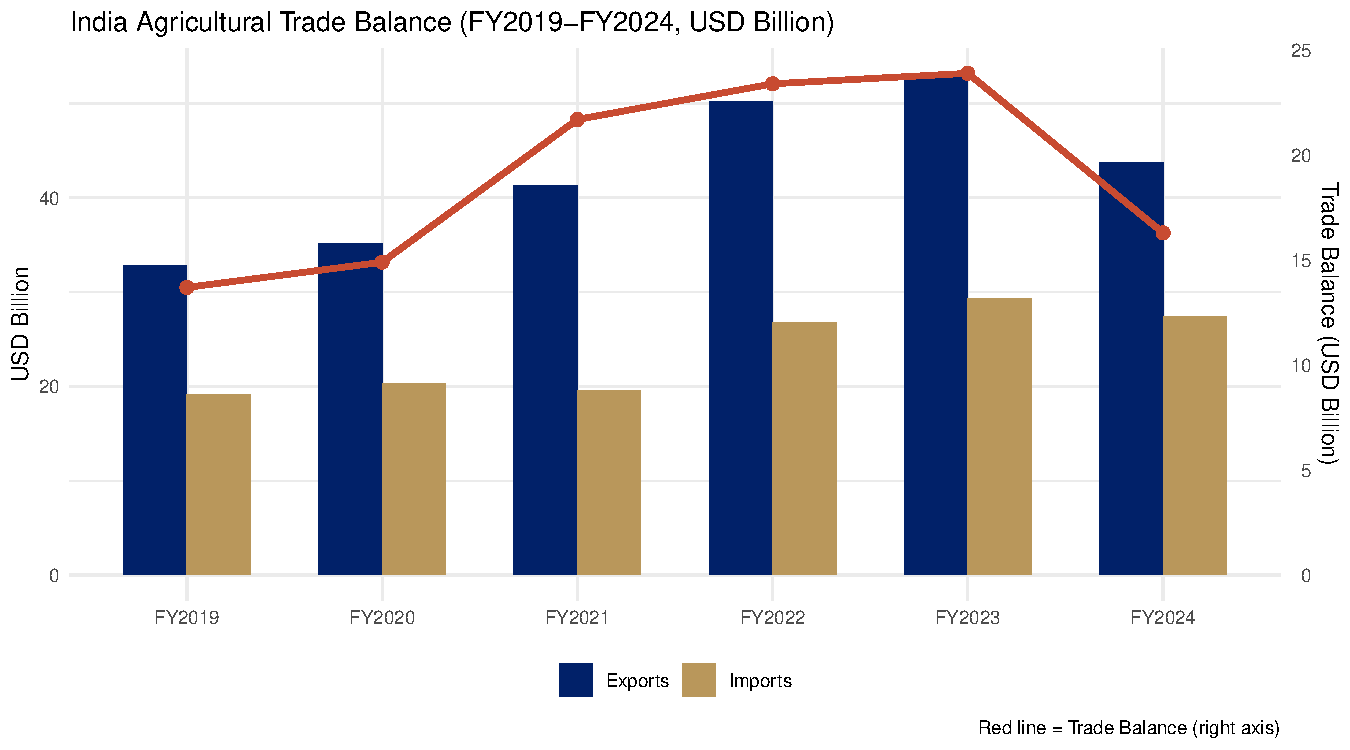
\includegraphics[keepaspectratio]{Lecture14_Agreement_on_Agriculture_files/figure-beamer/fig-india-agri-trade-1.pdf}}

}

\caption{\label{fig-india-agri-trade}India Agricultural Trade Balance
(FY2019-FY2024, USD Billion) Source: APEDA / DGCI\&S.}

\end{figure}%
\end{frame}

\begin{frame}{Key Takeaways: Agreement on Agriculture}
\phantomsection\label{key-takeaways-agreement-on-agriculture}
\textbf{Seven Things to Remember from Lecture 14}

\begin{enumerate}
\item
  \textbf{AoA has three pillars:} Market Access (tariffication + TRQs +
  reductions), Domestic Support (Green/Blue/Amber Boxes + de minimis),
  Export Competition (subsidy disciplines)
\item
  \textbf{India's bound tariffs average 113.5\%} --- the ``water'' in
  the tariff is India's primary agricultural protection instrument
\item
  \textbf{Three Boxes:} Green = unlimited (research, extension,
  decoupled payments); Blue = conditional (production-limiting); Amber =
  limited by de minimis (MSP procurement falls here)
\item
  \textbf{India's MSP procurement for rice likely exceeds 10\% de
  minimis} --- protected only by the Peace Clause (Bali 2013)
\item
  \textbf{FERP is the core injustice:} Using 1986--88 world prices
  (depressed by US/EU subsidies) overstates India's trade distortion.
  Updating FERP to current prices would solve India's problem
\item
  \textbf{Nairobi 2015 eliminated export subsidies} --- a genuine WTO
  success; India's RoDTEP is a legitimate tax refund scheme (if
  correctly calibrated)
\item
  \textbf{Doha Round dead} --- but AoA framework remains; India must
  push for permanent public stockholding solution at every MC
\end{enumerate}
\end{frame}

\begin{frame}{Next Lecture: SPS Measures and Codex Alimentarius}
\phantomsection\label{next-lecture-sps-measures-and-codex-alimentarius}
\begin{columns}[T]
\begin{column}{0.6\linewidth}
\textbf{Lecture 15 (August 4, 2026):}

\textbf{SPS Measures and Codex Alimentarius}

Why Indian spices were pulled from Singapore supermarkets.Why India's
shrimp face detention in the USA. Why EU pesticide standards block
Indian rice exports.

We will cover:

\begin{itemize}
\tightlist
\item
  \textbf{SPS Agreement} --- scientific basis, Codex/OIE/IPPC
\item
  \textbf{Codex Alimentarius} --- the food code that governs market
  access
\item
  \textbf{India's export rejection challenges:} spices, shrimp, basmati
  rice
\item
  \textbf{Case studies:} MDH/Everest spice scandal, Indian aquaculture
\item
  \textbf{India's strategy} for SPS compliance
\end{itemize}
\end{column}

\begin{column}{0.4\linewidth}
\textbf{Think About This}

In April 2023, \textbf{MDH and Everest} --- two of India's most iconic
spice brands --- had their products banned in Singapore and Hong Kong.

The reason: ethylene oxide (a fumigant) detected above permitted limits.

\emph{What standard did they violate? Who sets these standards? Is this
genuine food safety --- or disguised protectionism?}

We will answer all of these in Lecture 15.

\textbf{Reading:} - WTO SPS Agreement (full text) - FSSAI Annual Report
2023-24 - Spices Board of India Export Statistics - MPEDA: Aquaculture
Export Performance Report
\end{column}
\end{columns}
\end{frame}

\section{Appendix}\label{appendix}

\begin{frame}{Additional Resources}
\phantomsection\label{additional-resources}
\begin{columns}[T]
\begin{column}{0.5\linewidth}
\textbf{Further Reading}

\begin{itemize}
\tightlist
\item
  \emph{International Economics} --- Salvatore (Ch. 12)
\item
  \emph{International Economics} --- Appleyard \& Field (Ch. 12)
\item
  RBI/DGCI\&S/APEDA databases for latest data
\end{itemize}
\end{column}

\begin{column}{0.5\linewidth}
\textbf{Key Data Sources}

\begin{itemize}
\tightlist
\item
  DGCI\&S: India's merchandise trade
\item
  RBI: Balance of payments data\\
\item
  APEDA: Agricultural export statistics
\item
  WTO: Tariff and trade databases
\end{itemize}
\end{column}
\end{columns}
\end{frame}




\end{document}
